\documentclass[11pt,graphicx,caption,rotating]{article}
\textheight=24cm
\textwidth=18cm
\topmargin=-2cm
\oddsidemargin=0cm
\usepackage[utf8x]{inputenc}
%\usepackage[latin1]{inputenc}
\usepackage[activeacute,spanish]{babel}
\usepackage{amssymb,amsfonts}
\usepackage[tbtags]{amsmath}
\usepackage{pict2e}
\usepackage{ucs}
\usepackage{float}
\usepackage[all]{xy}
\usepackage{graphics,graphicx,color,colortbl}
\usepackage{times}
\usepackage{subfigure}
\usepackage{wrapfig}
\usepackage{multicol}
\usepackage{cite}
\usepackage{url}
\usepackage[tbtags]{amsmath}
\usepackage{amsmath,amssymb,amsfonts,amsbsy}
\usepackage{bm}
\usepackage{algorithm}
\usepackage{algorithmic}
\usepackage[centerlast, small]{caption}
\usepackage[colorlinks=true, citecolor=black, linkcolor=black, urlcolor=black,breaklinks=true]{hyperref}
\hyphenation{ele-men-tos he-rra-mi-en-ta cons-tru-yen trans-fe-ren-ci-a pro-pu-es-tas si-mu-lar vi-sua-li-za-cion}

\begin{document}
\title{\textbf{Compuerta NAND en tecnología AMI}}
\author{David Ricardo Martínez Hernández}
\date{}
\maketitle
\noindent
Se requiere realizar el diseño y simulación de la celda estándar para una compuerta NAND a través del software Electric, basándose en la tecnología AMI y considerando $t_r=3t_f$.

\section{Diseño}
\noindent
Para realizar la compuerta NAND en la tecnología AMI en Electric sera utilizada la libreria \textit{C5models}.\\
La ecu(\ref{ecu1}) que definen el tiempo de subida es
\begin{equation}
 t_r = k'_p\frac{L_pC_L}{W_p}
\label{ecu1}
\end{equation}
\noindent
La ecu(\ref{ecu2}) que definen el tiempo de bajada es
\begin{equation}
 t_f = k'_n\frac{L_nC_L}{W_n}
\label{ecu2}
\end{equation}
\noindent
Donde:\\
$C_L$  es la capaitancia de salida.\\
$k'$ es el parámetro de transconductancia para cada transistor.\\
$W$ es el ancho del transistor.\\
$L$ es el largo del transistor.\\\\
El parámetro de transconductancia del proceso para cada transistor se define en ecu.(\ref{ecu3}) y ecu.(\ref{ecu4}):
\begin{equation}
 k'_p =  \mu _p C_{OX} = \mu _p \frac{t_{OX}}{\varepsilon _{Si O_2} }
 \label{ecu3}
\end{equation}
\begin{equation}
 k'_n =  \mu _n C_{OX} = \mu _n \frac{t_{OX}}{\varepsilon _{Si O_2} }
 \label{ecu4}
\end{equation}
\noindent
Donde:\\
$t_{OX}$ es el ancho del óxido del transistor.\\
$\varepsilon _{SiO_2}$ es la permitividad del óxido de silicio.\\
$\mu$ es la movilidad de huecos electrones según corresponda.\\\\
Los tiempos se obtienen de ecu.(\ref{ecu5}):
\begin{equation}
 \mu _p \frac{t_{OX}}{\varepsilon _{SiO_2}} \frac{L_pC_L}{W_p}  = 3 \mu _n \frac{t_{OX}}{\varepsilon _{SiO_2}} \frac{L_nC_L}{W_n}
 \label{ecu5}
\end{equation}
\noindent
De acuerdo a la tecnología de diseño se tiene que:\\
$\mu _p = 212.0166131\, [cm^2/s]$.\\
$\mu _n = 458.939679\, [cm^2/s]$.\\\\
Al despejar $W_p$ en función de $W_n$ de la ecu.(\ref{ecu5}) se obtiene:
\begin{equation}
 W_p = 0.154158 W_n
 \label{ecu6}
\end{equation}
\noindent
Para el diseño del layout a una escala de $300\, nm$ se tomó el largo mínimo que es $0.6\, \mu m$, es decir $L=2$, $W_p = 5$, reemplazando el valor de $W_p$ en la ecu.(\ref{ecu6}) se obtiene que $W_n = 32.43$.

\section{Simulación}
\noindent
Se implemento el layout de la compuerta NAND en electric como se observa en la Figura~\ref{fig1}.
\begin{figure}[H]
  \centering
    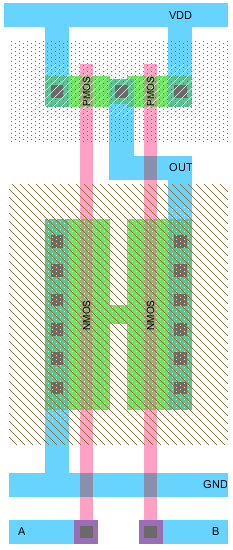
\includegraphics[scale=0.5]{fig1.png}
      \caption{Layout de la compuerta NAND en electric.}
  \label{fig1}
\end{figure}
\noindent
Se realizaron las simulaciones para verificar el correcto funcionamiento de la compuerta por medio de LTSPICE, mostrando los resultados obtenidos en la figuras~\ref{fig2}, \ref{fig3} y \ref{fig4}.
\begin{figure}[H]
  \centering
    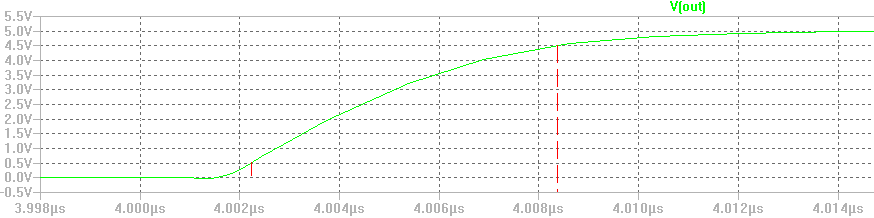
\includegraphics[scale=0.5]{fig2.png}
      \caption{Simulación del tiempo de subida para la compuerta NAND en LTSPICE.}
  \label{fig2}
\end{figure}
\begin{figure}[H]
  \centering
    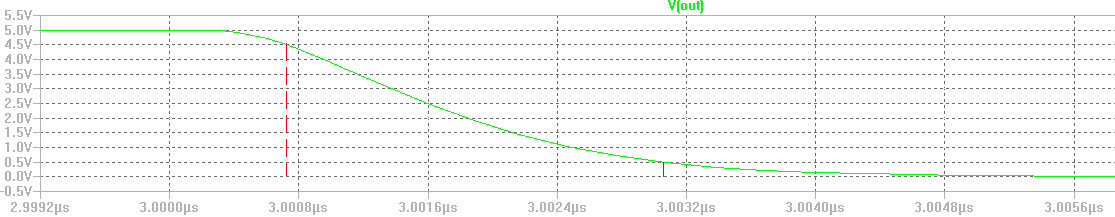
\includegraphics[scale=0.4]{fig3.png}
      \caption{Simulación del tiempo de bajada para la compuerta NAND en LTSPICE.}
  \label{fig3}
\end{figure}
\begin{figure}[H]
  \centering
    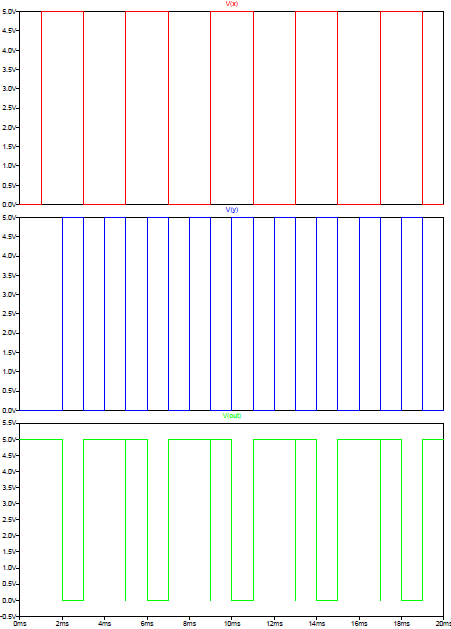
\includegraphics[scale=0.5]{fig4.png}
      \caption{Simulación del funcionamiento de la compuerta NAND.}
  \label{fig4}
\end{figure}


\end{document}